						 
\begin{frame}{\citetitle{MapaRealidadVirtual_UPV_2022}$^*$  (1)}
\begin{columns}
\begin{column}{0.99\textwidth}
	\begin{itemize}
		\item Se propone una aplicación de RA que despliegue un MAPA de la UPV
		\item Se generó el modelo utilizando Blender y se exportó a un formato GLB
		\item La aplicación hace uso de la cámara para desplegar el modelo en una superficie con textura
	\end{itemize}
\end{column}
\begin{column}{0.01\textwidth}  
\begin{center}
     \begin{tabular}{c}
%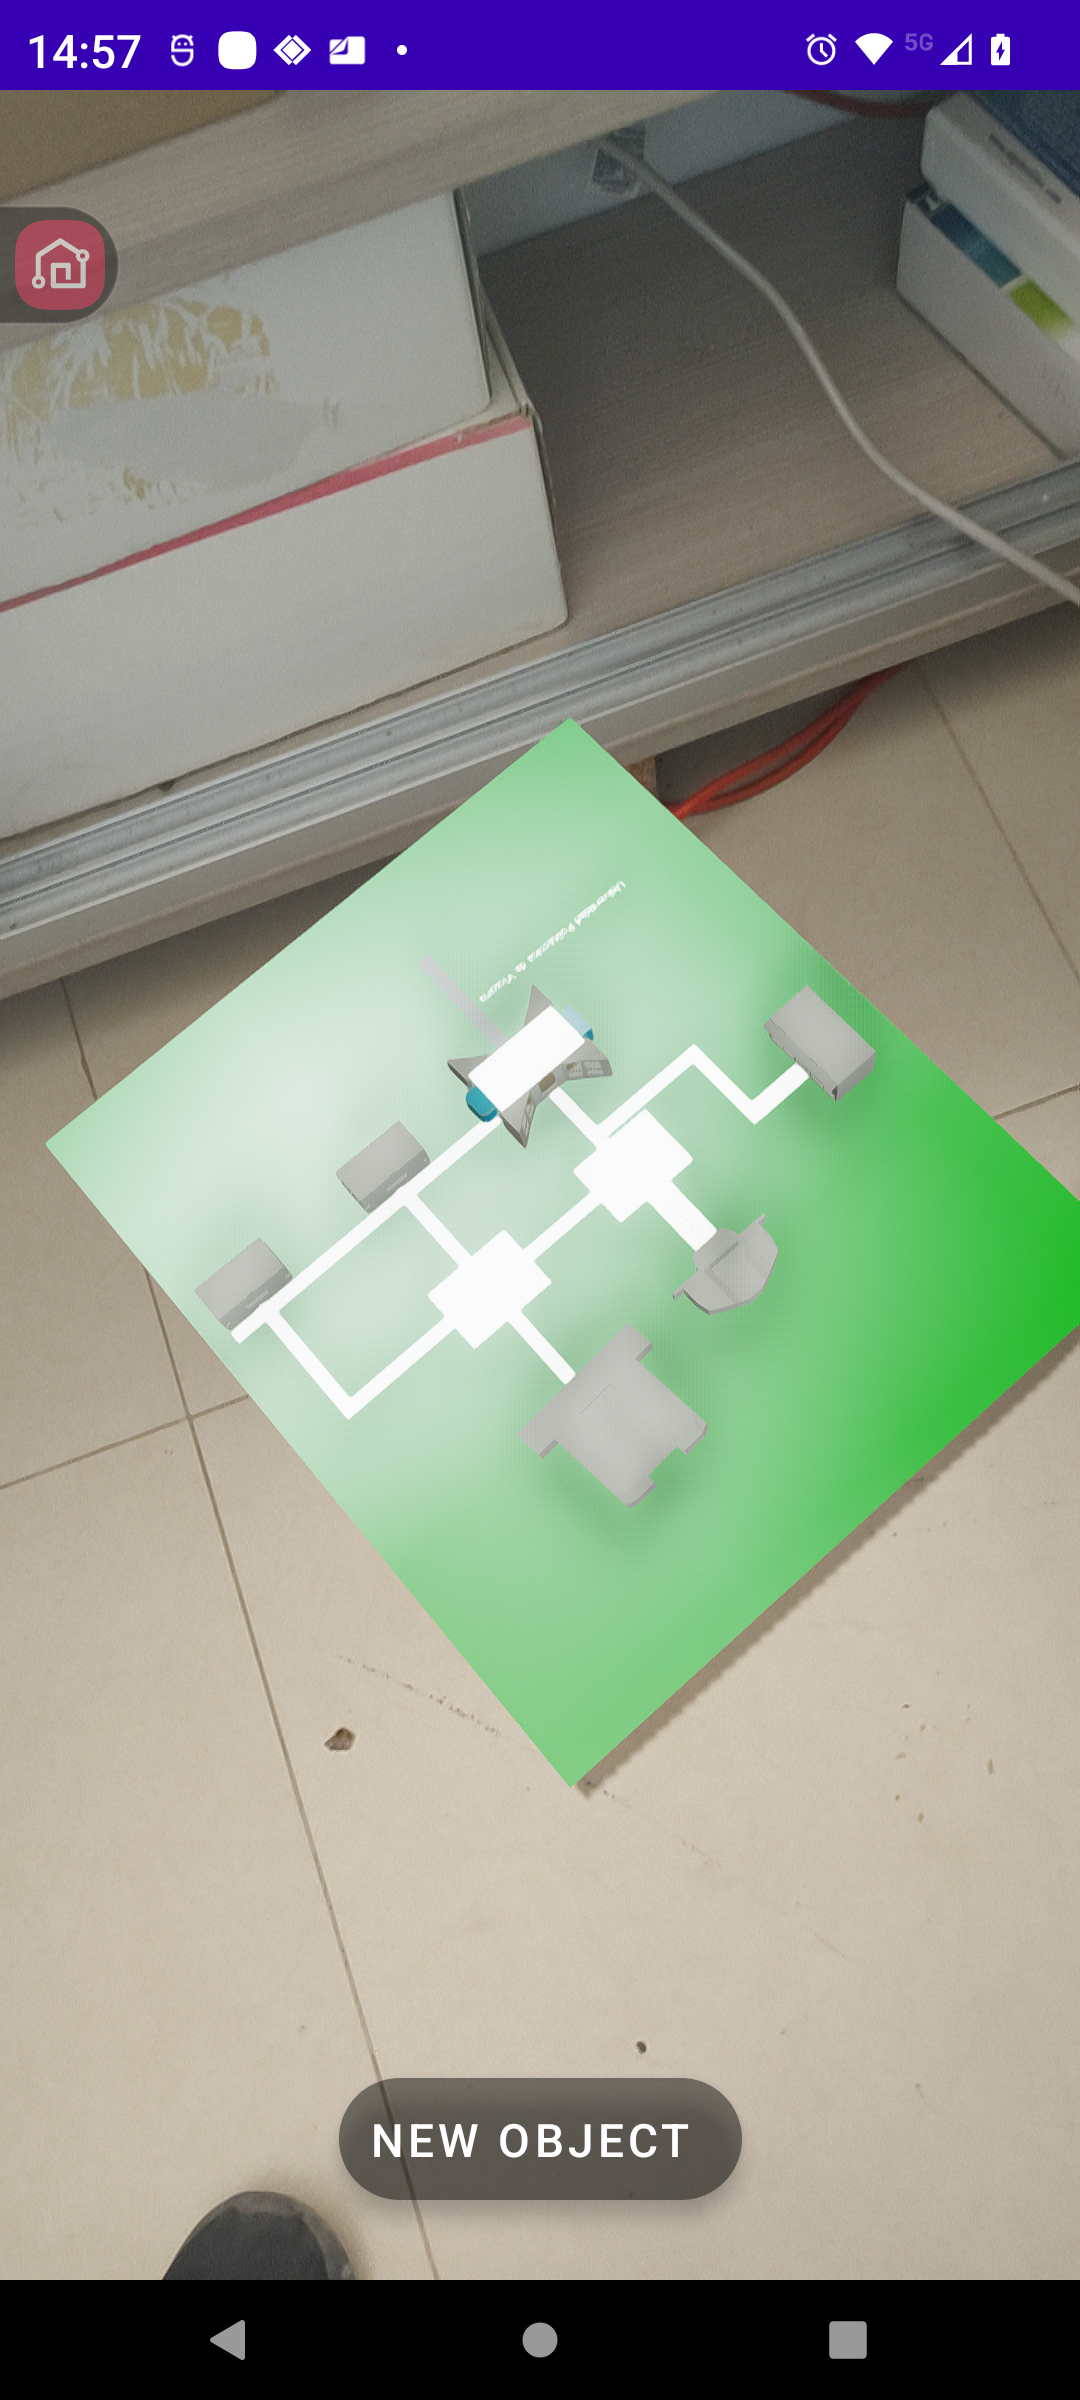
\includegraphics[width=0.48\textwidth]{2022_MapaUPV_RealidadAumentada/figs/MapaUPV_01}
%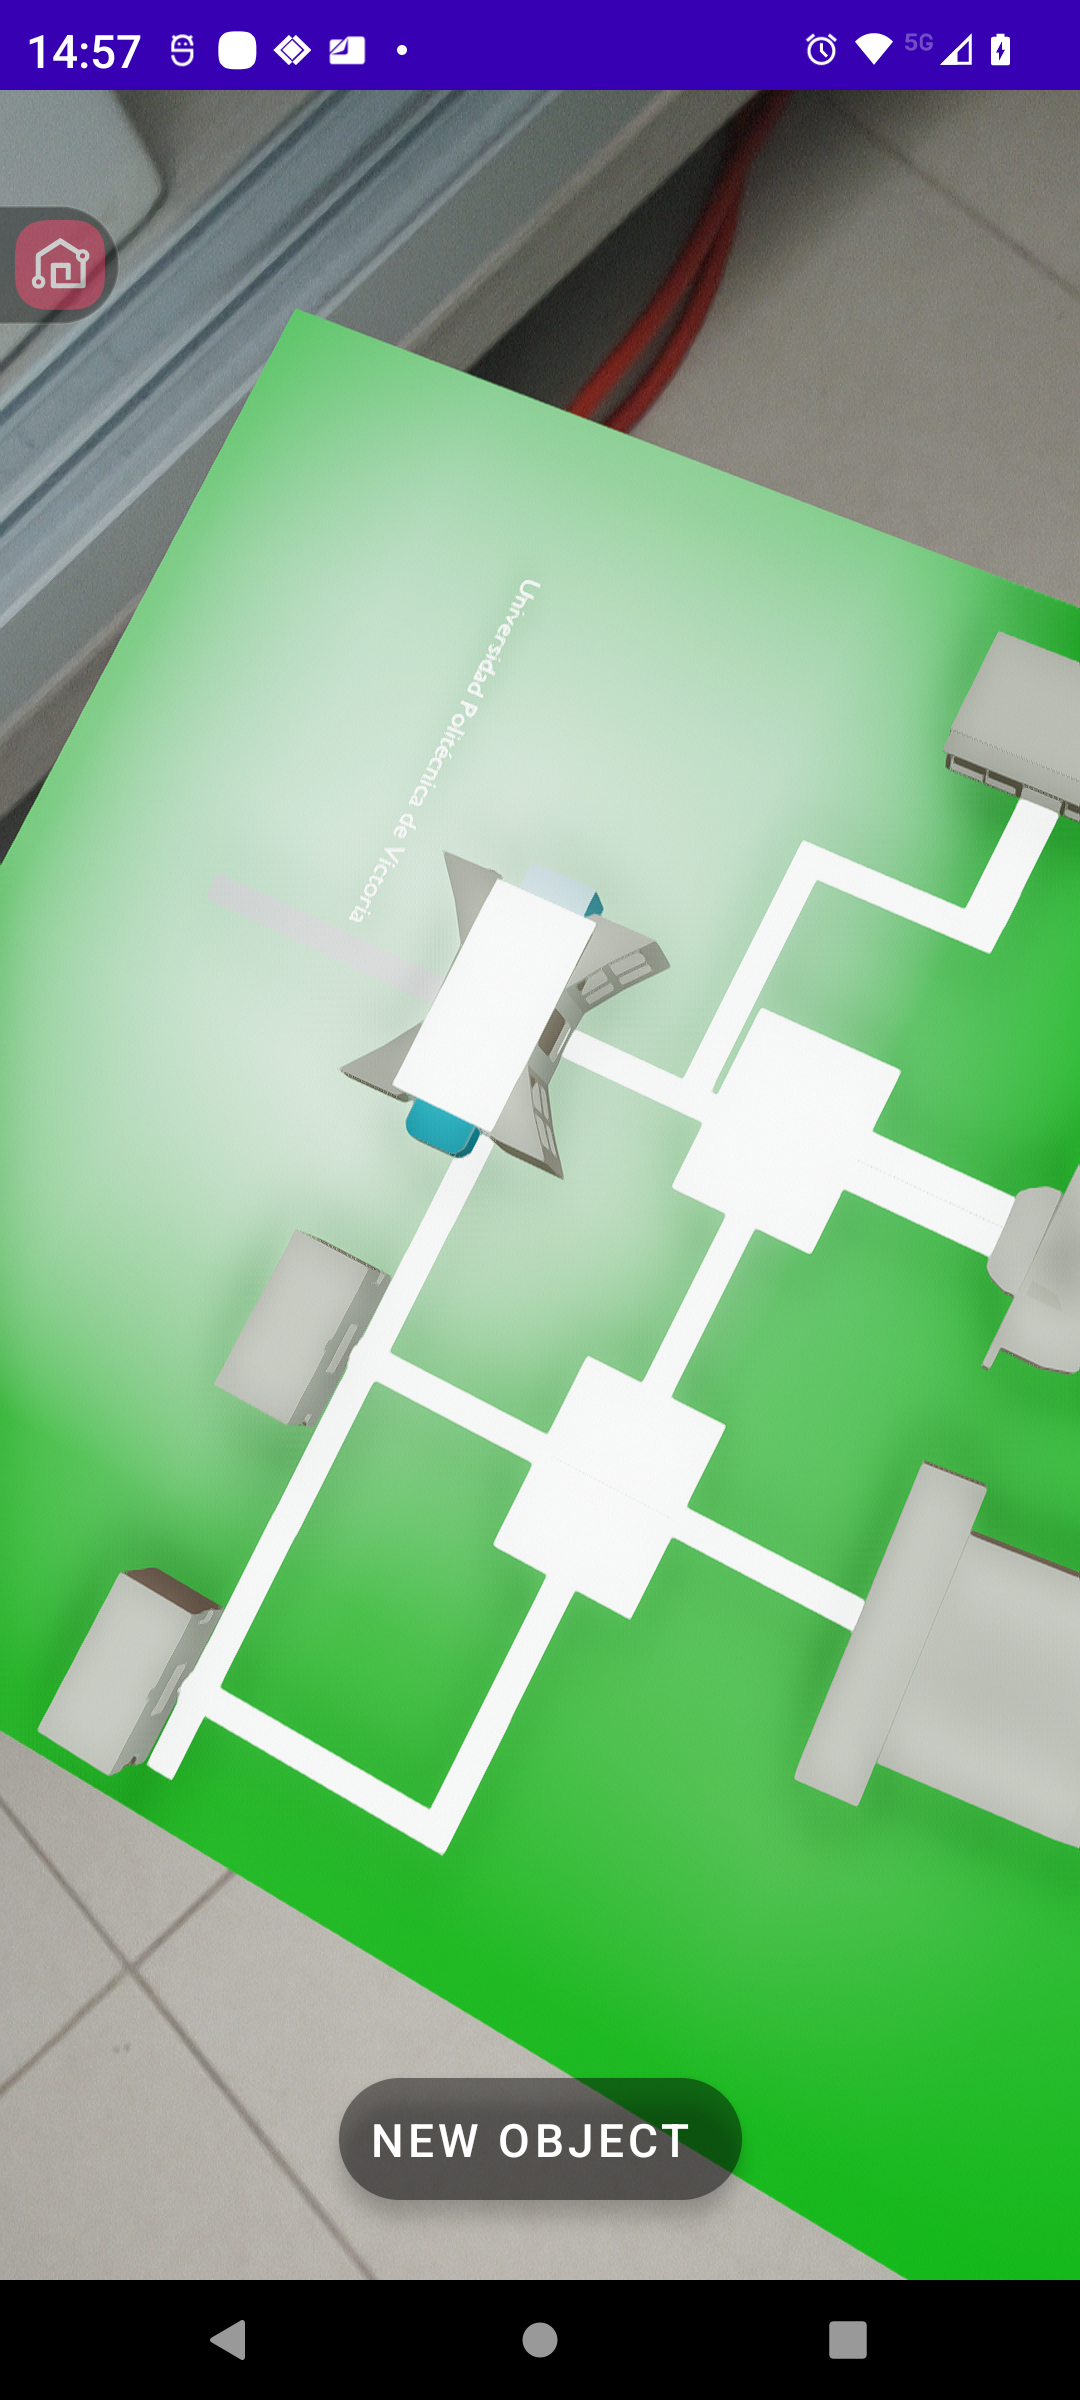
\includegraphics[width=0.48\textwidth]{2022_MapaUPV_RealidadAumentada/figs/MapaUPV_02}\\         
      \end{tabular}
\end{center}
\end{column} 
\end{columns} 
\footfullcite*{MapaRealidadVirtual_UPV_2022}
\end{frame}


\begin{frame}{\citetitle{MapaRealidadVirtual_UPV_2022}  (2)}
\begin{columns}
\begin{column}{0.4\textwidth}
	\begin{itemize}
		\item Se propone una aplicación de RA que despliegue un MAPA de la UPV
	\end{itemize}
\end{column}
\begin{column}{0.6\textwidth}  
\begin{center}
     \begin{tabular}{c}
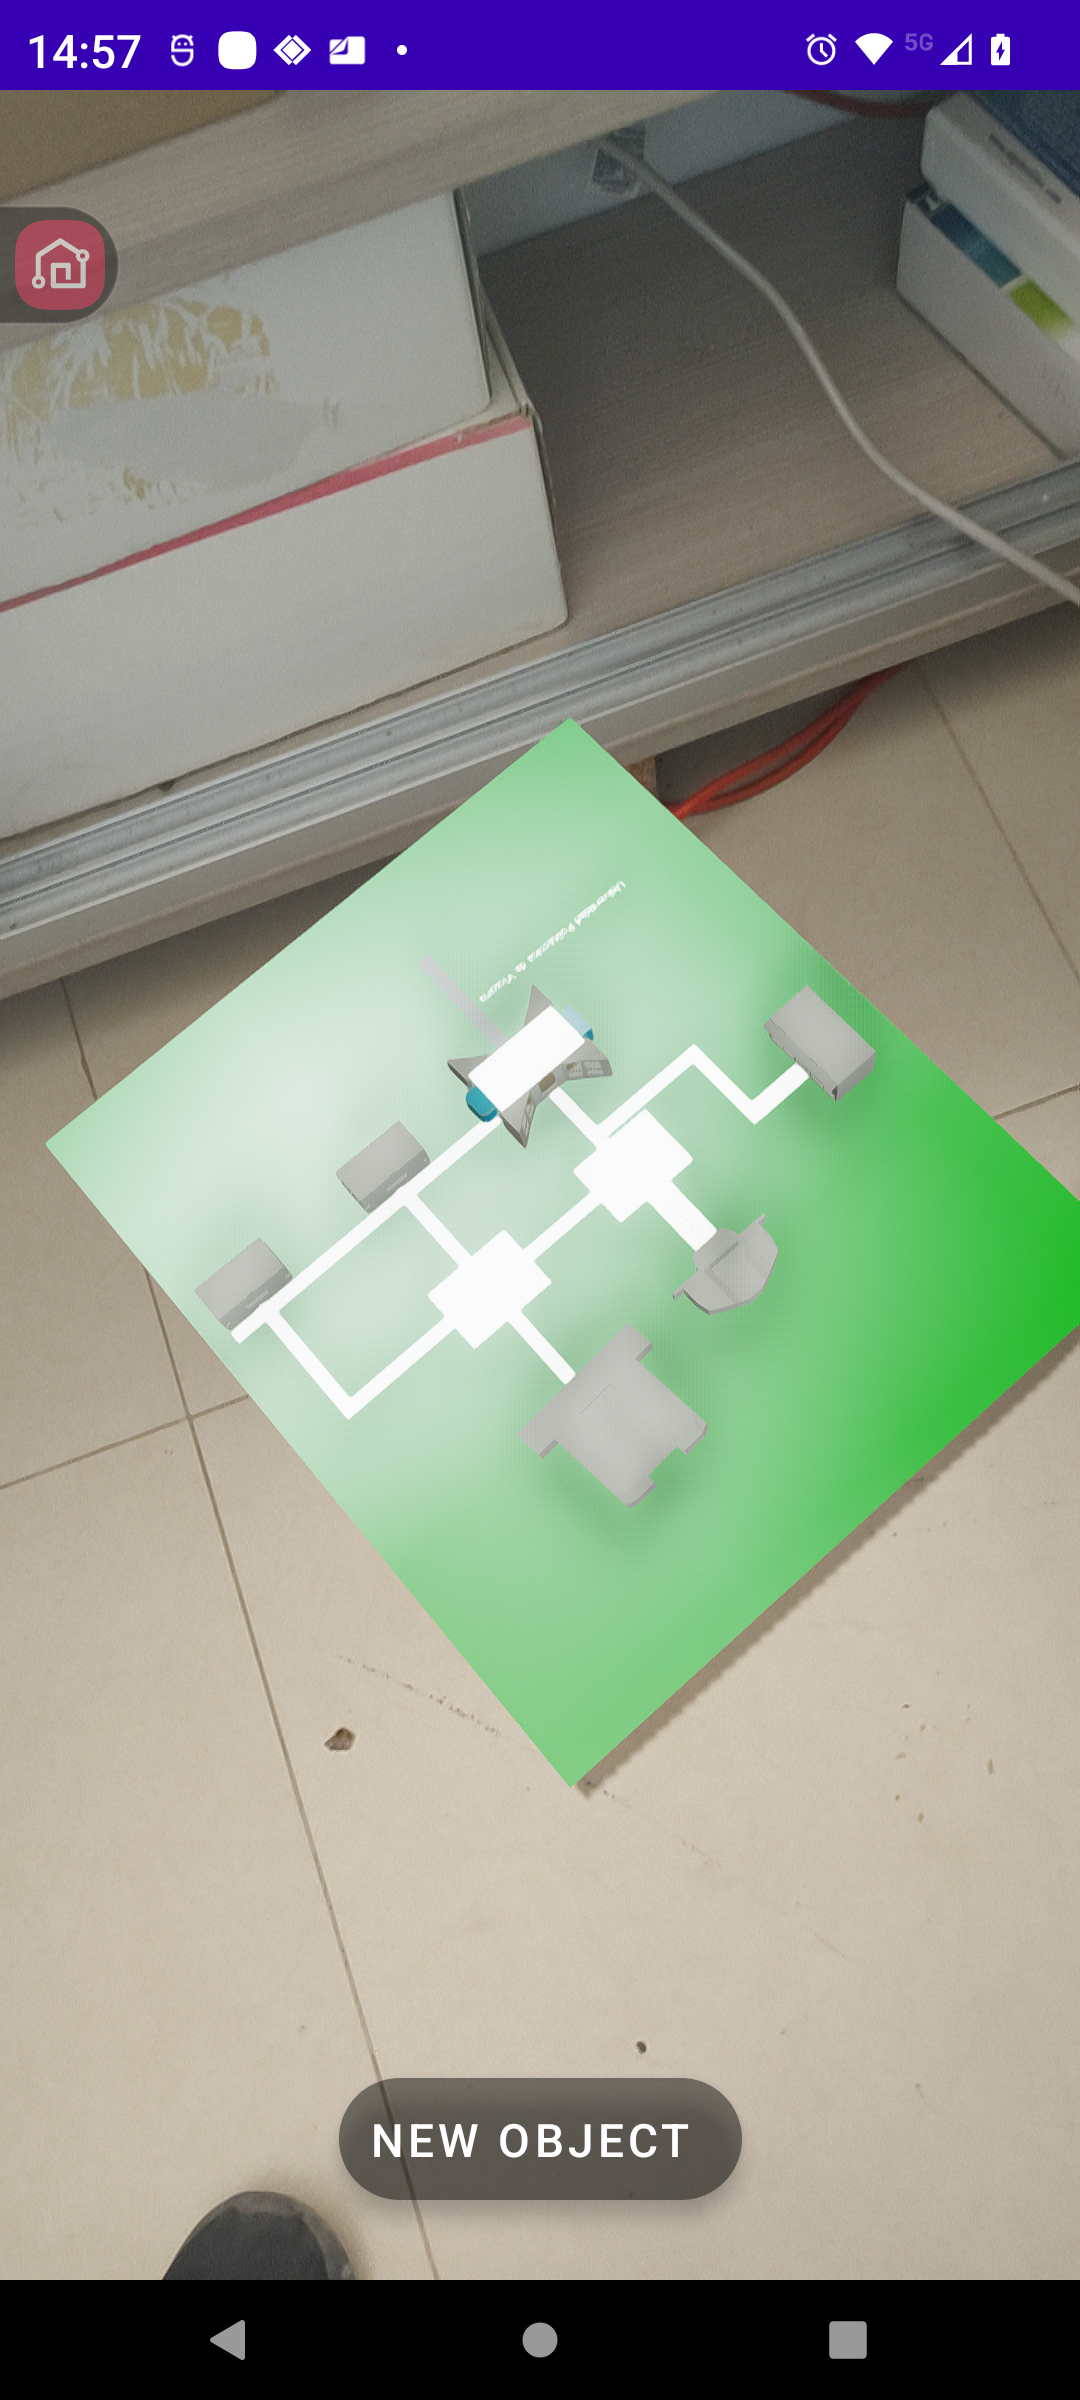
\includegraphics[width=0.24\textwidth]{2022_MapaUPV_RealidadAumentada/figs/MapaUPV_01}
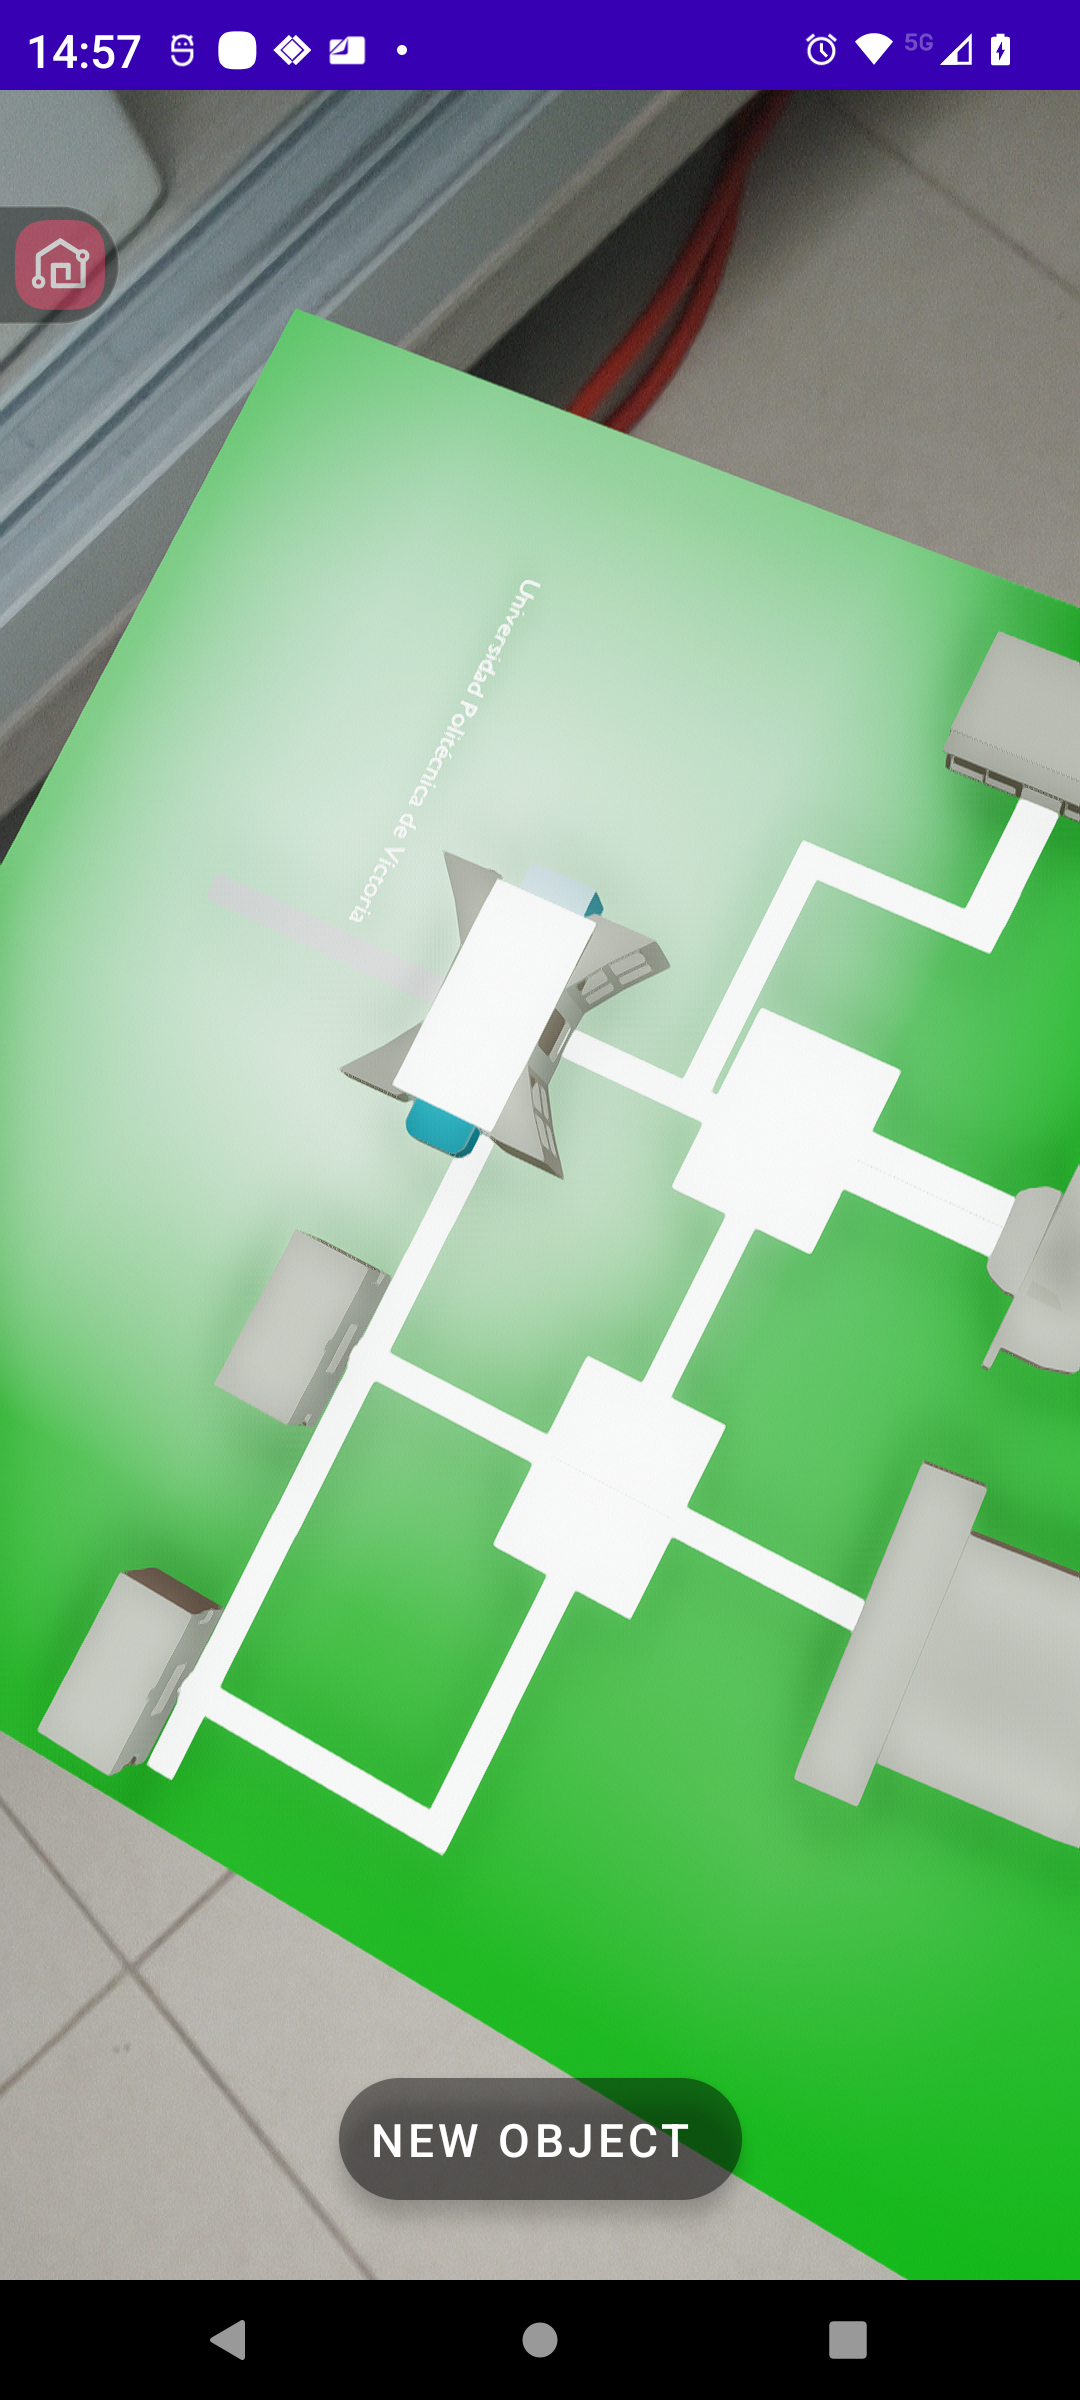
\includegraphics[width=0.24\textwidth]{2022_MapaUPV_RealidadAumentada/figs/MapaUPV_02}
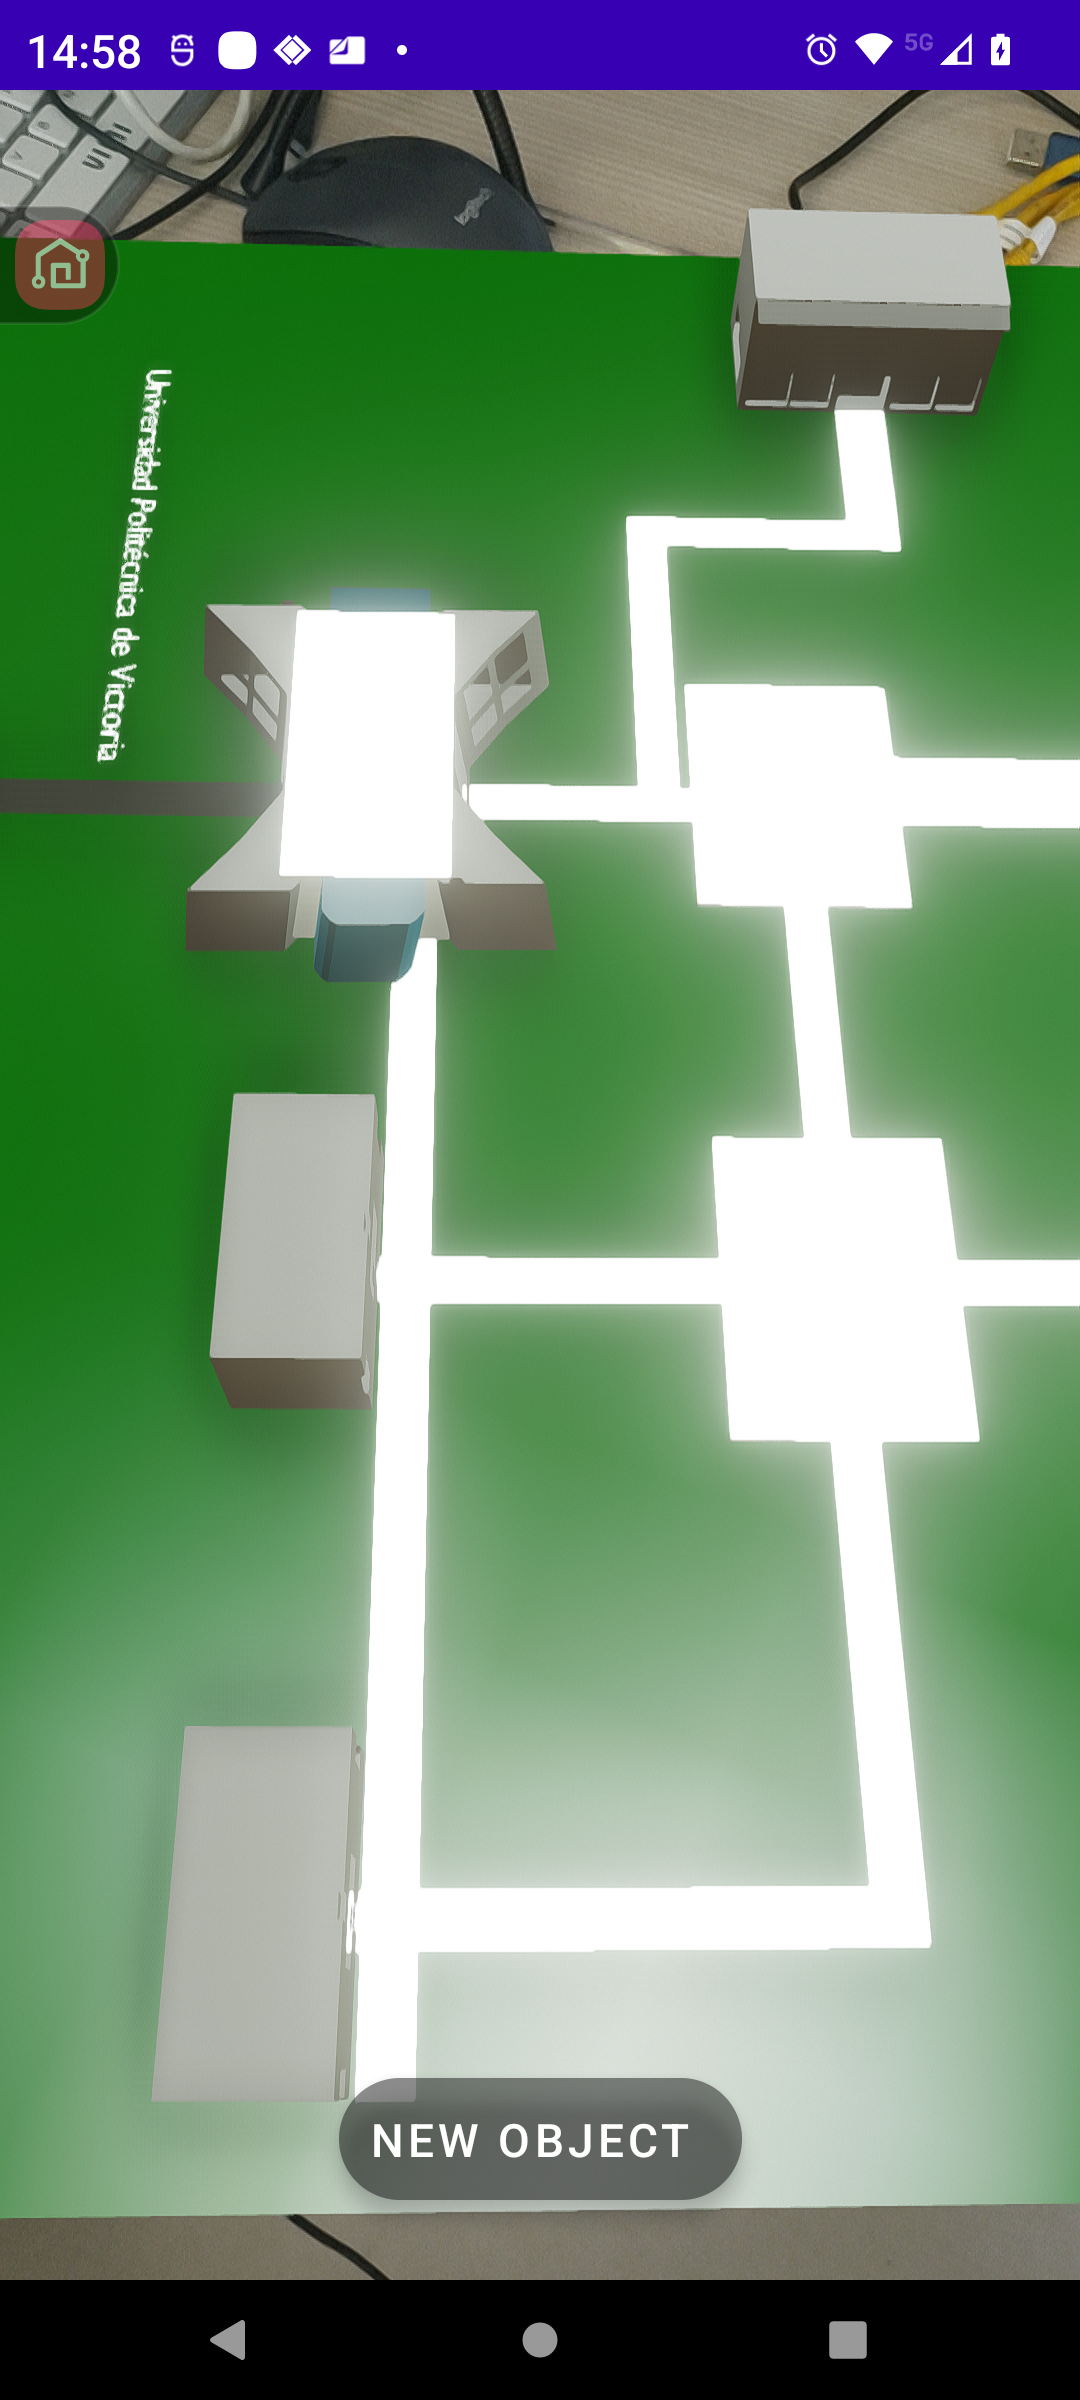
\includegraphics[width=0.24\textwidth]{2022_MapaUPV_RealidadAumentada/figs/MapaUPV_03}
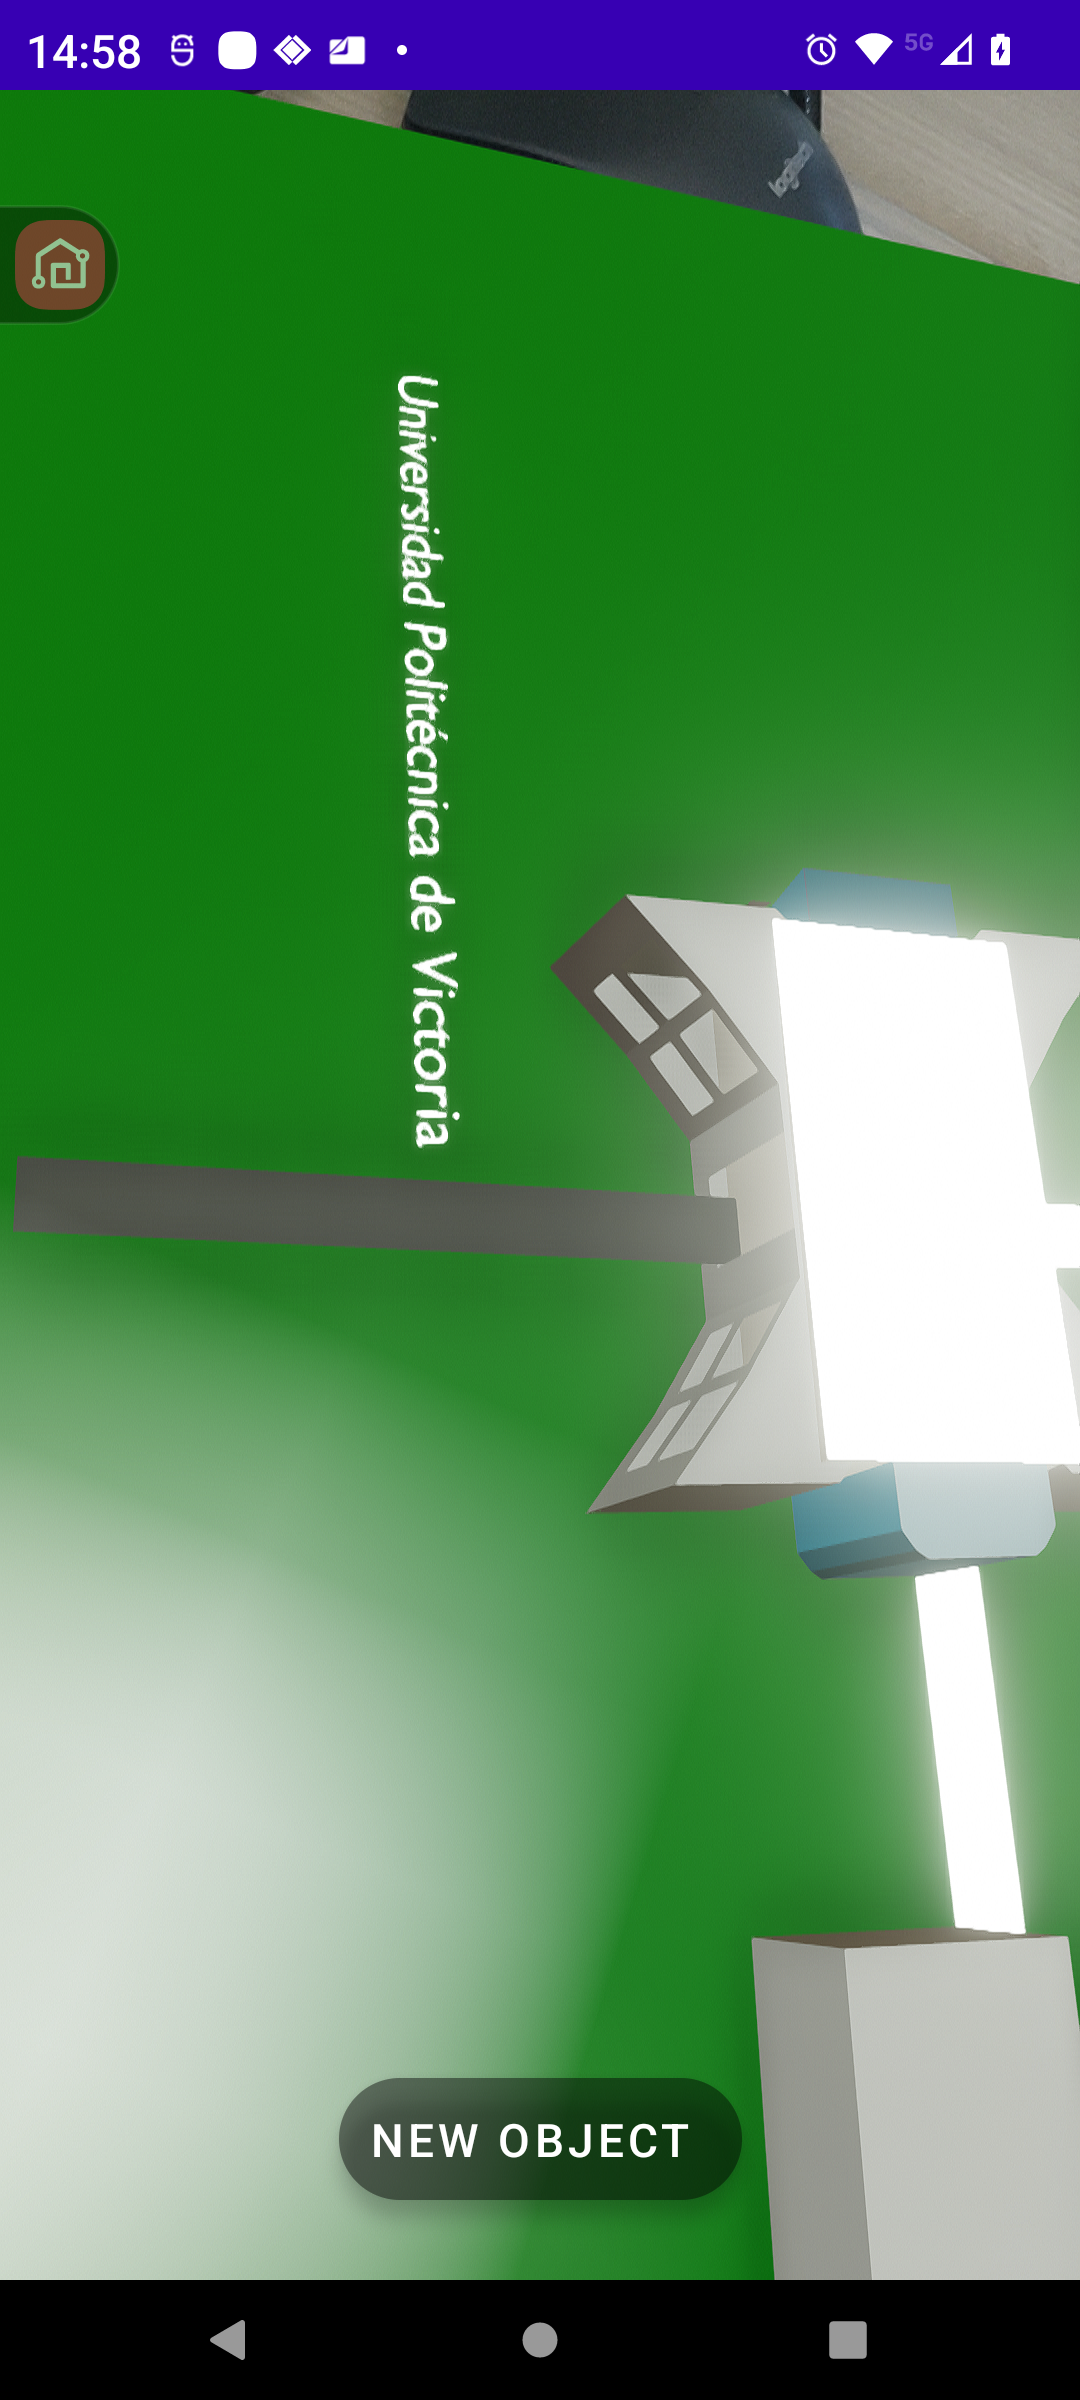
\includegraphics[width=0.24\textwidth]{2022_MapaUPV_RealidadAumentada/figs/MapaUPV_04}\\         
      \end{tabular}
\end{center}
\end{column} 
\end{columns} 

\end{frame}





